\begin{homeworkProblem}

\textbf{Required: OpenAI Spinning Up in Deep RL}. Welcome to \href{https://spinningup.openai.com/en/latest/user/introduction.html}{Spinning Up in Deep RL}! This is an educational resource produced by OpenAI that makes it easier to learn about deep reinforcement learning (deep RL). Please study the documents and install the environment with PyTorch version.

(a) Finish the problem set 1: ``\href{https://spinningup.openai.com/en/latest/spinningup/exercises.html#problem-set-1-basics-of-implementation}{Basics of Implementation}". It includes three exercises: Gaussian Log-Likelihood, Policy for PPO, and Computation Graph for TD3.

(b) Finish the problem set 2: ``\href{https://spinningup.openai.com/en/latest/spinningup/exercises.html#problem-set-2-algorithm-failure-modes}{Algorithm Failure Modes}". It includes two exercises: Value Function Fitting in TRPO, and Silent Bug in DDPG.

\solution

(a) After setting up the environment in the methods in `README.md', we can successfully run the codes. The codes cuold be check in `code/spinningup/spinup/exercises/pytorch/problem\_set\_1'.

\begin{itemize}
    \item exercise 1\_1: For a $k$ dimension diagnoal Gaussian distribtion $\mathbf{x}\sim\N(\bmu,\bSigma)$, where $\bSigma=\diag(\sigma_1^2,\dots,\sigma_k^2)$, thus its PDF is
    $$p(\mathbf{x};\bmu,\bSigma)=\dfrac{1}{(2\pi)^{\frac{k}{2}}\,|\bSigma|^{\frac{1}{2}}}\exp\left[-\frac{1}{2}(\mathbf{x}-\bmu)^{\top}\bSigma^{-1}(\mathbf{x}\bmu)\right]$$
    Where
    $$|\bSigma|=\prod_{i=1}^{k}\sigma_i^{2}, \qquad \bSigma^{-1}=\diag\left(\sigma_1^{-2},\dots,\sigma_k^{-2}\right), \qquad (\mathbf{x}-\bmu)^{\top}\bSigma^{-1}(\mathbf{x}-\bmu)=\sum_{i=1}^{k}\frac{(x_i-\mu_i)^2}{\sigma_i^{2}}$$
    So above all, the log-likelihood is
    \begin{align*}
    \log p(\mathbf{x};\bmu,\bSigma) &= -\frac{k}{2}\log(2\pi)-\sum_{i=1}^{k}\log\sigma_i-\frac{1}{2}\sum_{i=1}^{k}\frac{(x_i-\mu_i)^2}{\sigma_i^{2}} \\
    &= -\dfrac{1}{2}\sum_{i=1}^k\left(\log(2\pi)+2\log\sigma_i+\left(\dfrac{x_i-\mu_i}{\sigma_i}\right)^2\right)
    \end{align*}

    The implementation are check results are as follows:
    \begin{figure}[h]
        \centering
        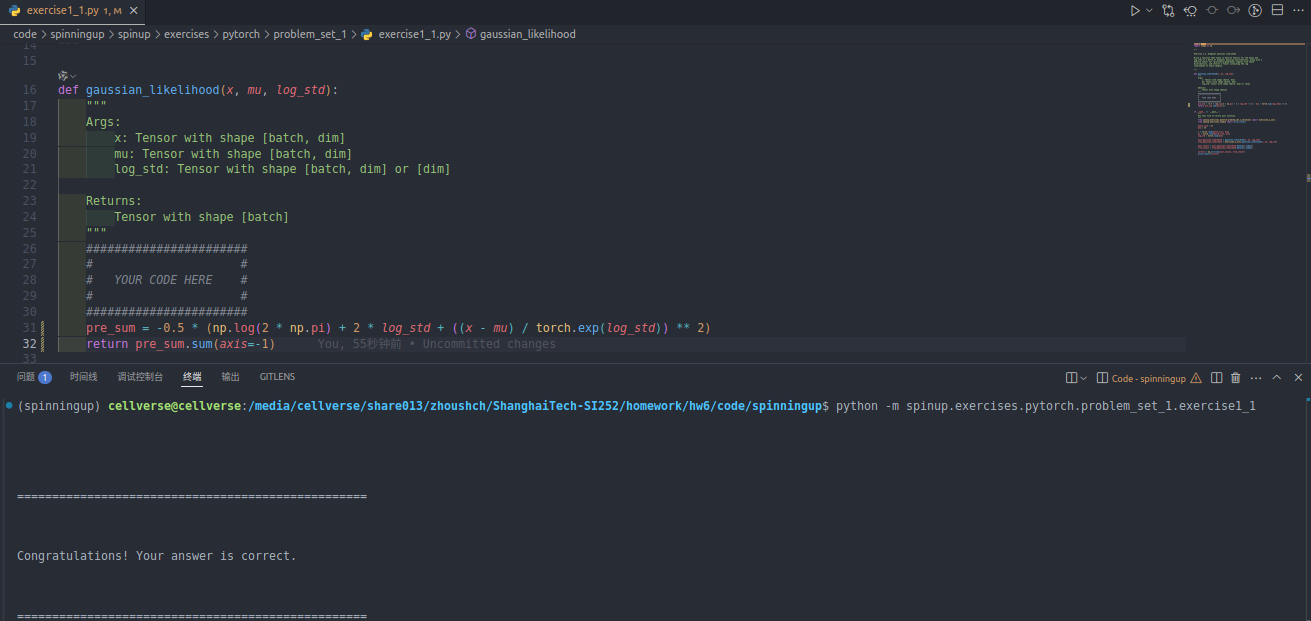
\includegraphics[width=\textwidth]{../Img/spinningup_exercises/1_1.png}
    \end{figure}

    \item exercise 1\_2: The implementation are check results are as follows:
    \begin{figure}[h]
        \centering
        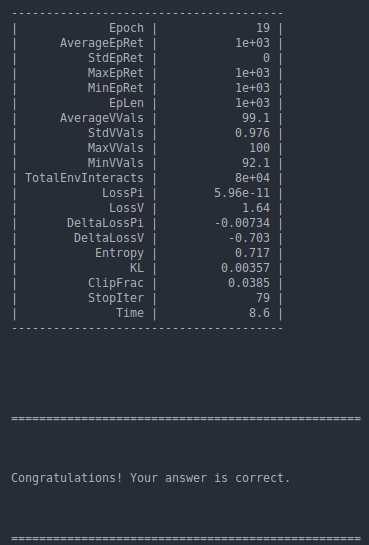
\includegraphics[width=0.5\textwidth]{../Img/spinningup_exercises/1_2.png}
    \end{figure}

    \item exercise 1\_3:
    According to the discription, within 10 rounds, the score in HalfSheetah should exceed 300, while the score in InvertedPendulum should reach 150.

    And the following curves show that the performance achieved the expected results:
    \begin{figure}[H]
        \centering
        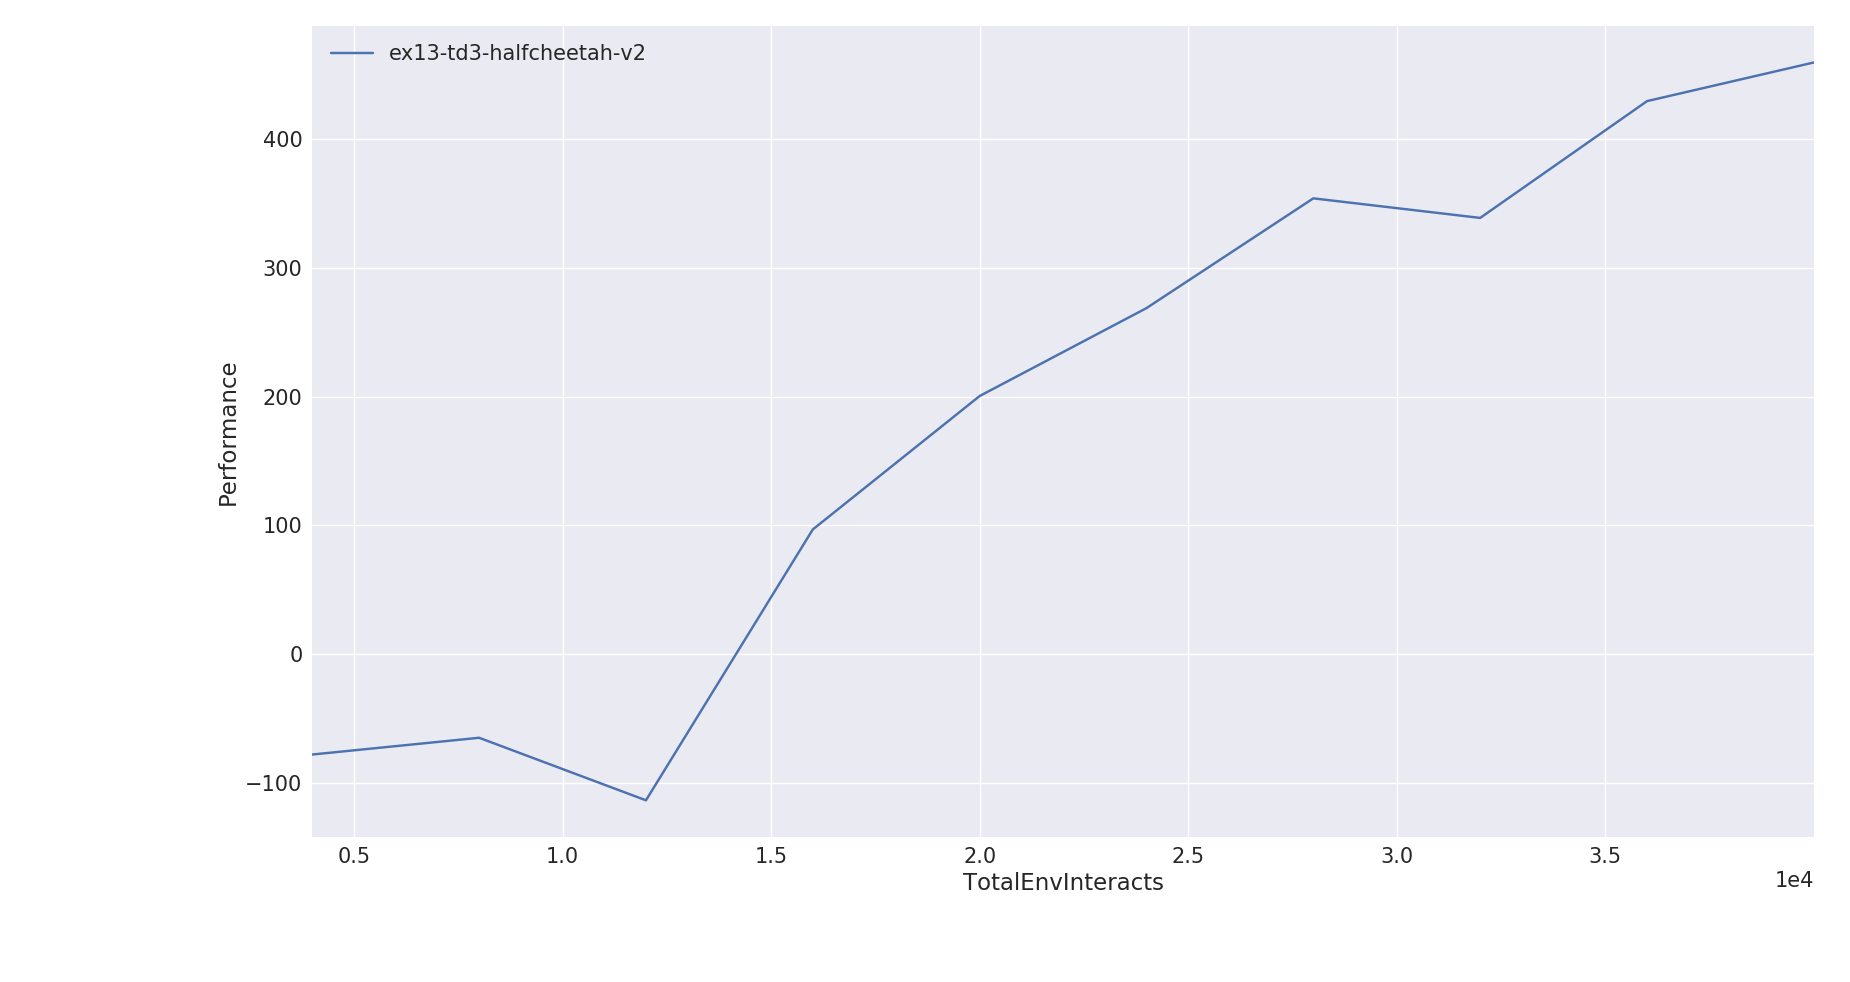
\includegraphics[width=\textwidth]{../Img/spinningup_exercises/1_3_healthcare.png}
        \vspace{-2cm}
    \end{figure}
    \begin{figure}[H]
        \centering
        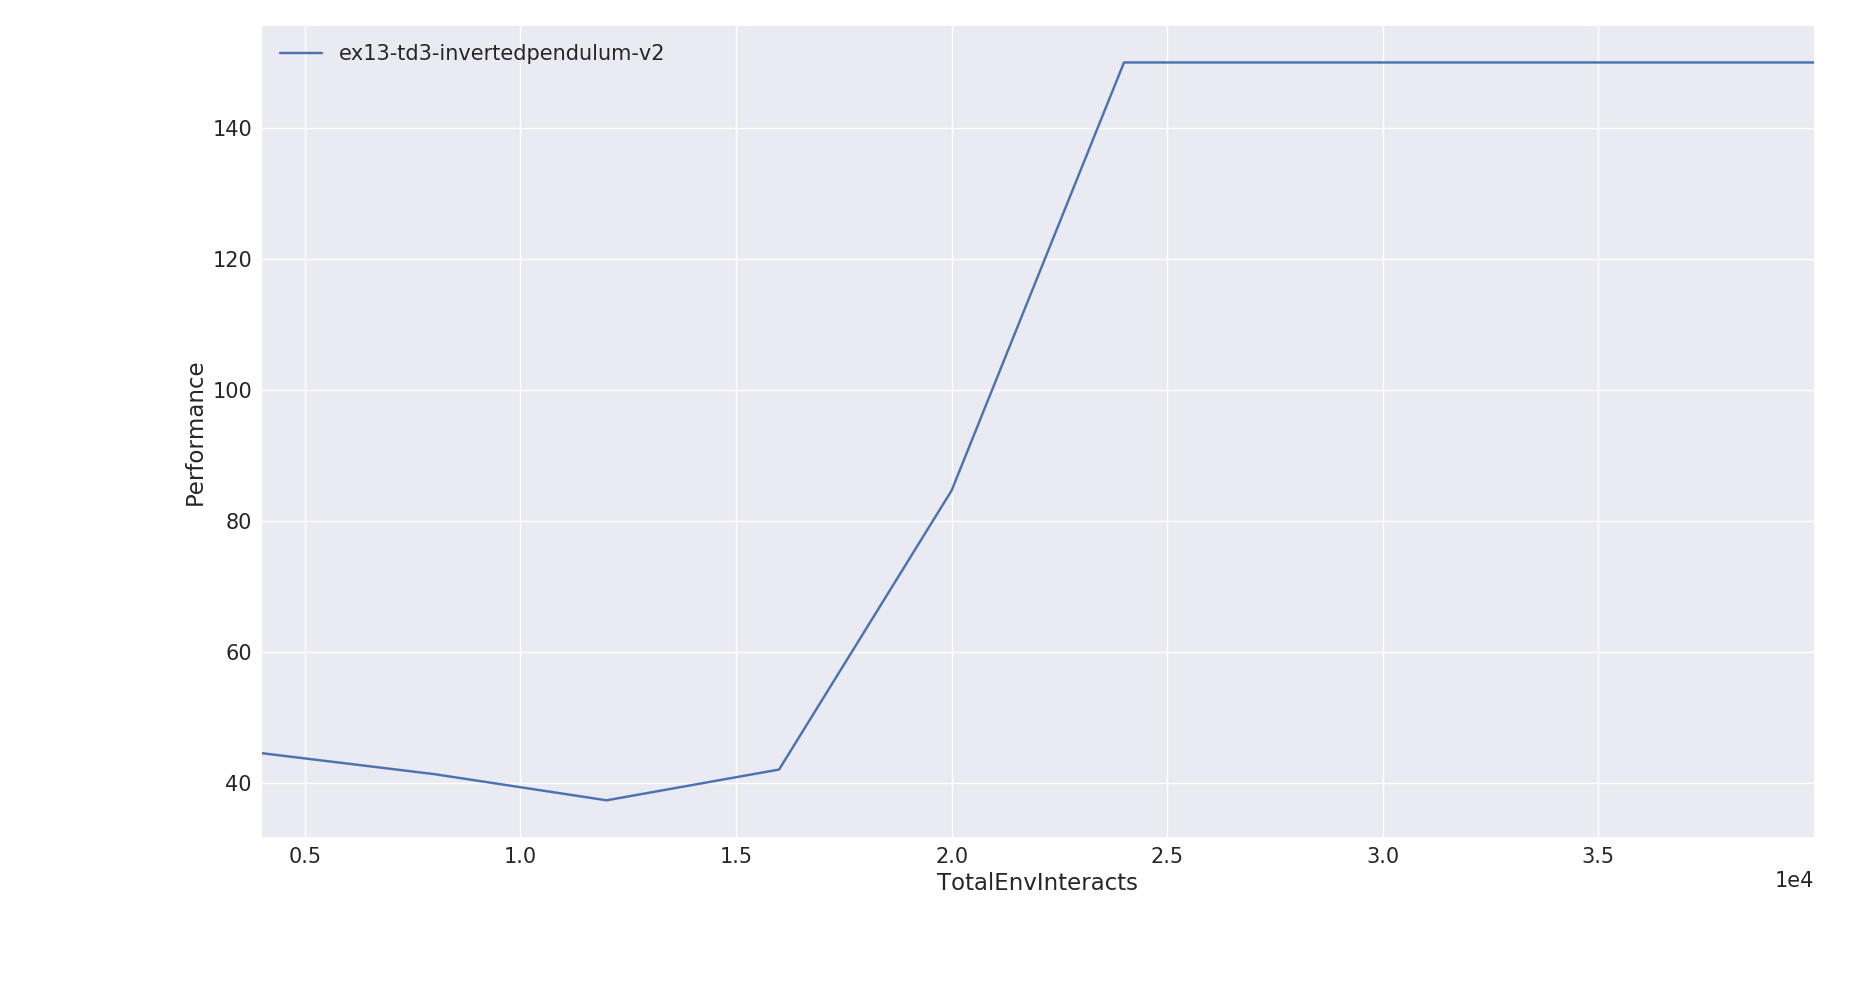
\includegraphics[width=\textwidth]{../Img/spinningup_exercises/1_3_invertedpendulum.png}
    \end{figure}

\end{itemize}


(b) Run the commands in the `README.md', we can get the following reults. The codes cuold be check in `code/spinningup/spinup/exercises/pytorch/problem\_set\_2'.

\begin{itemize}
    \item exercise 2\_1:

    The difference is quite substantial: with a trained value function, the agent is able to quickly make progress. With an untrained value function, the agent gets stuck early on.

    The curve of v0 with different seeds are as follows:
    \begin{figure}[H]
        \centering
        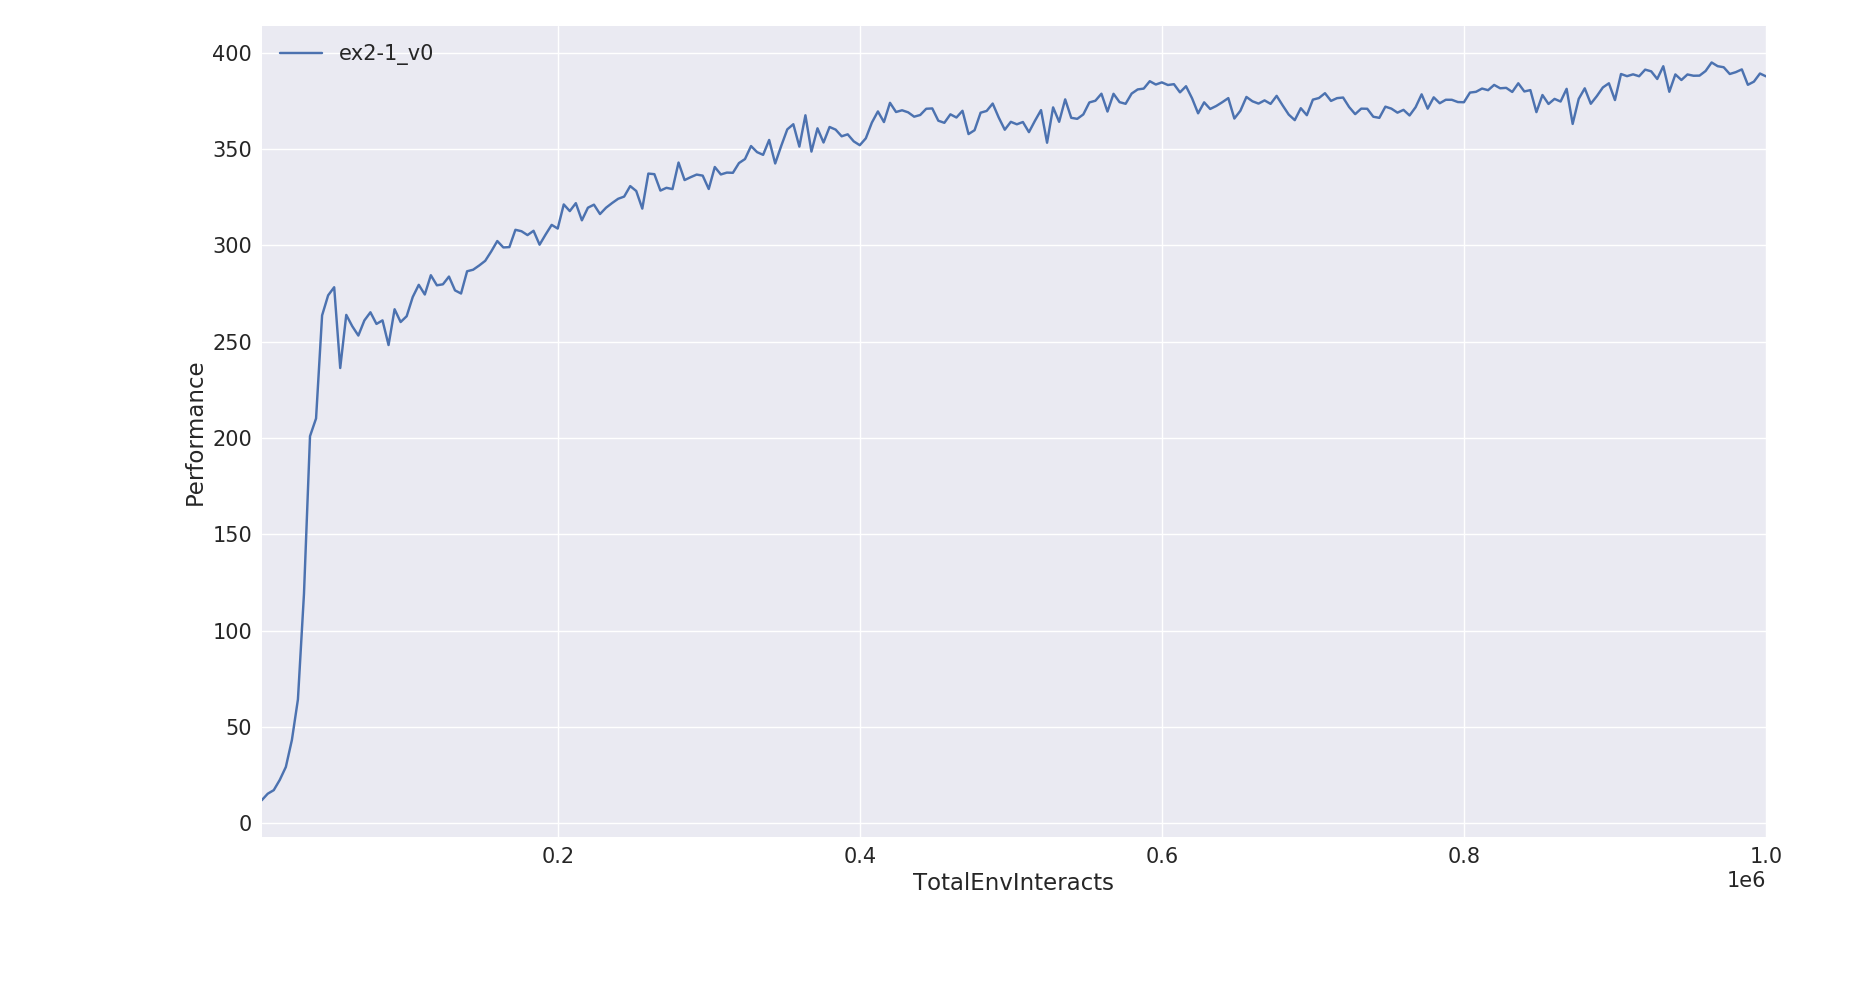
\includegraphics[width=0.32\textwidth]{../Img/spinningup_exercises/2_1/2_1_curve_v0_s0.png}
        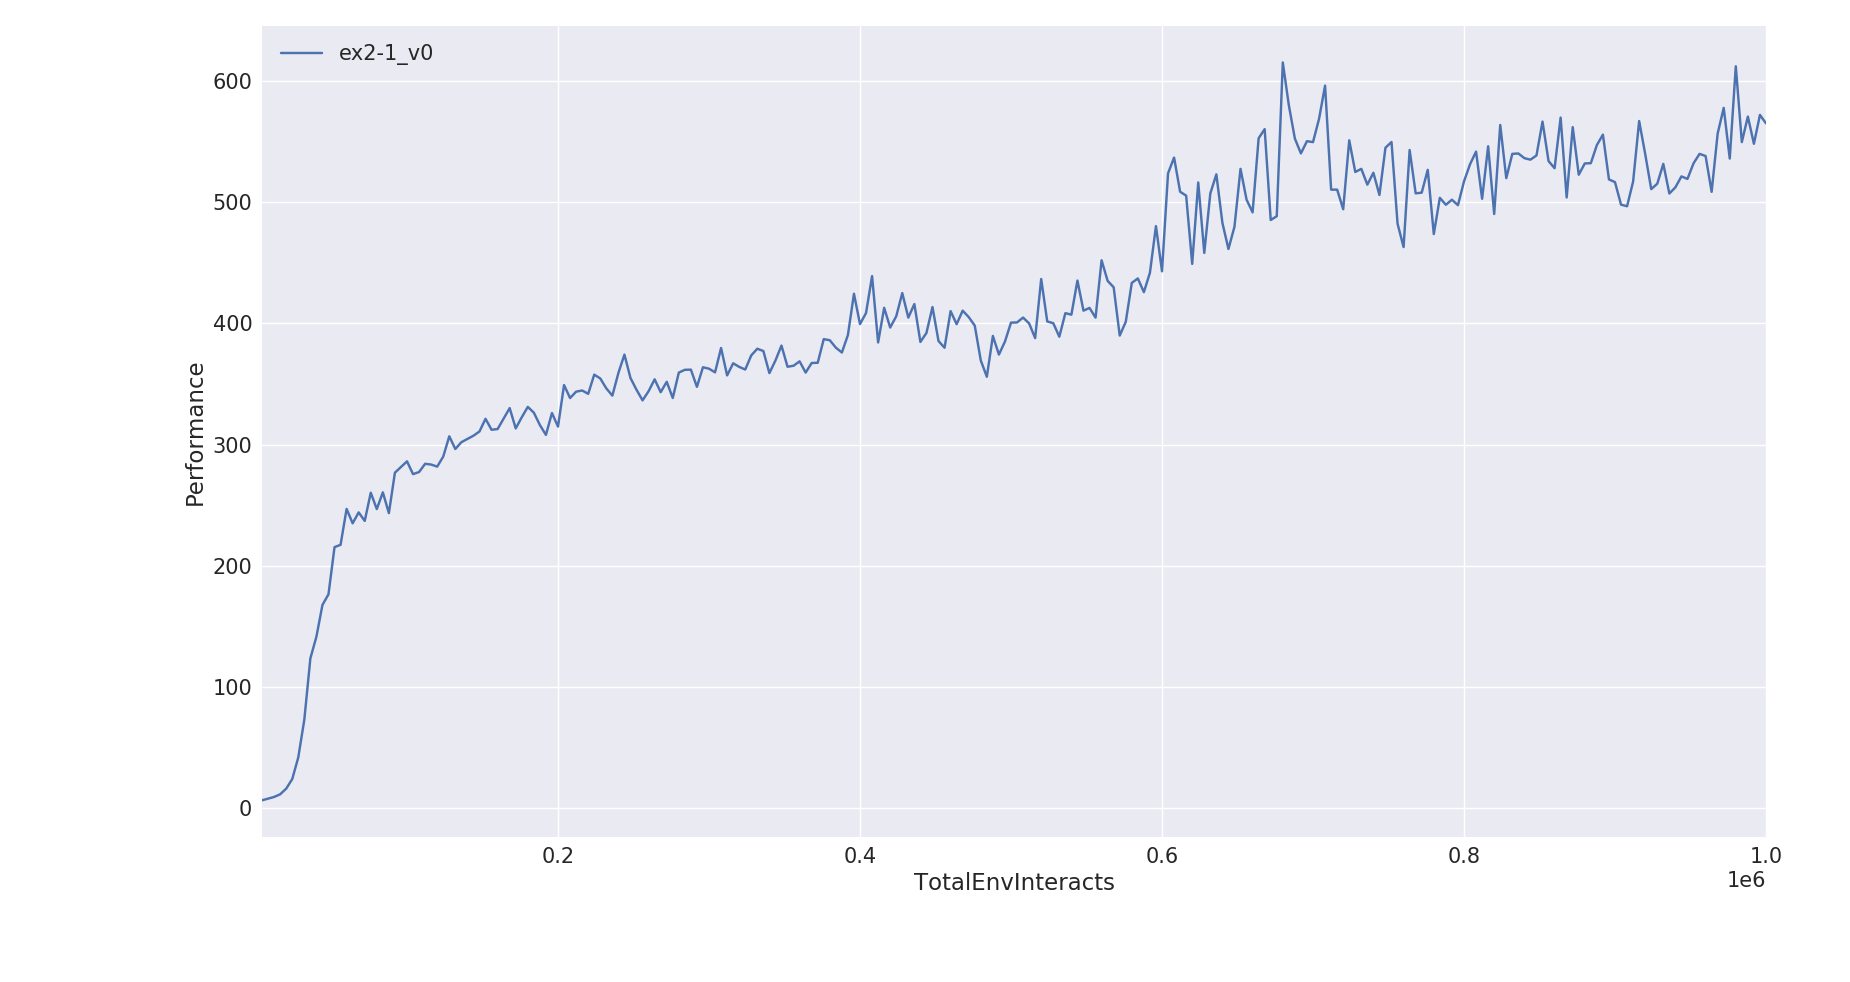
\includegraphics[width=0.32\textwidth]{../Img/spinningup_exercises/2_1/2_1_curve_v0_s10.png}
        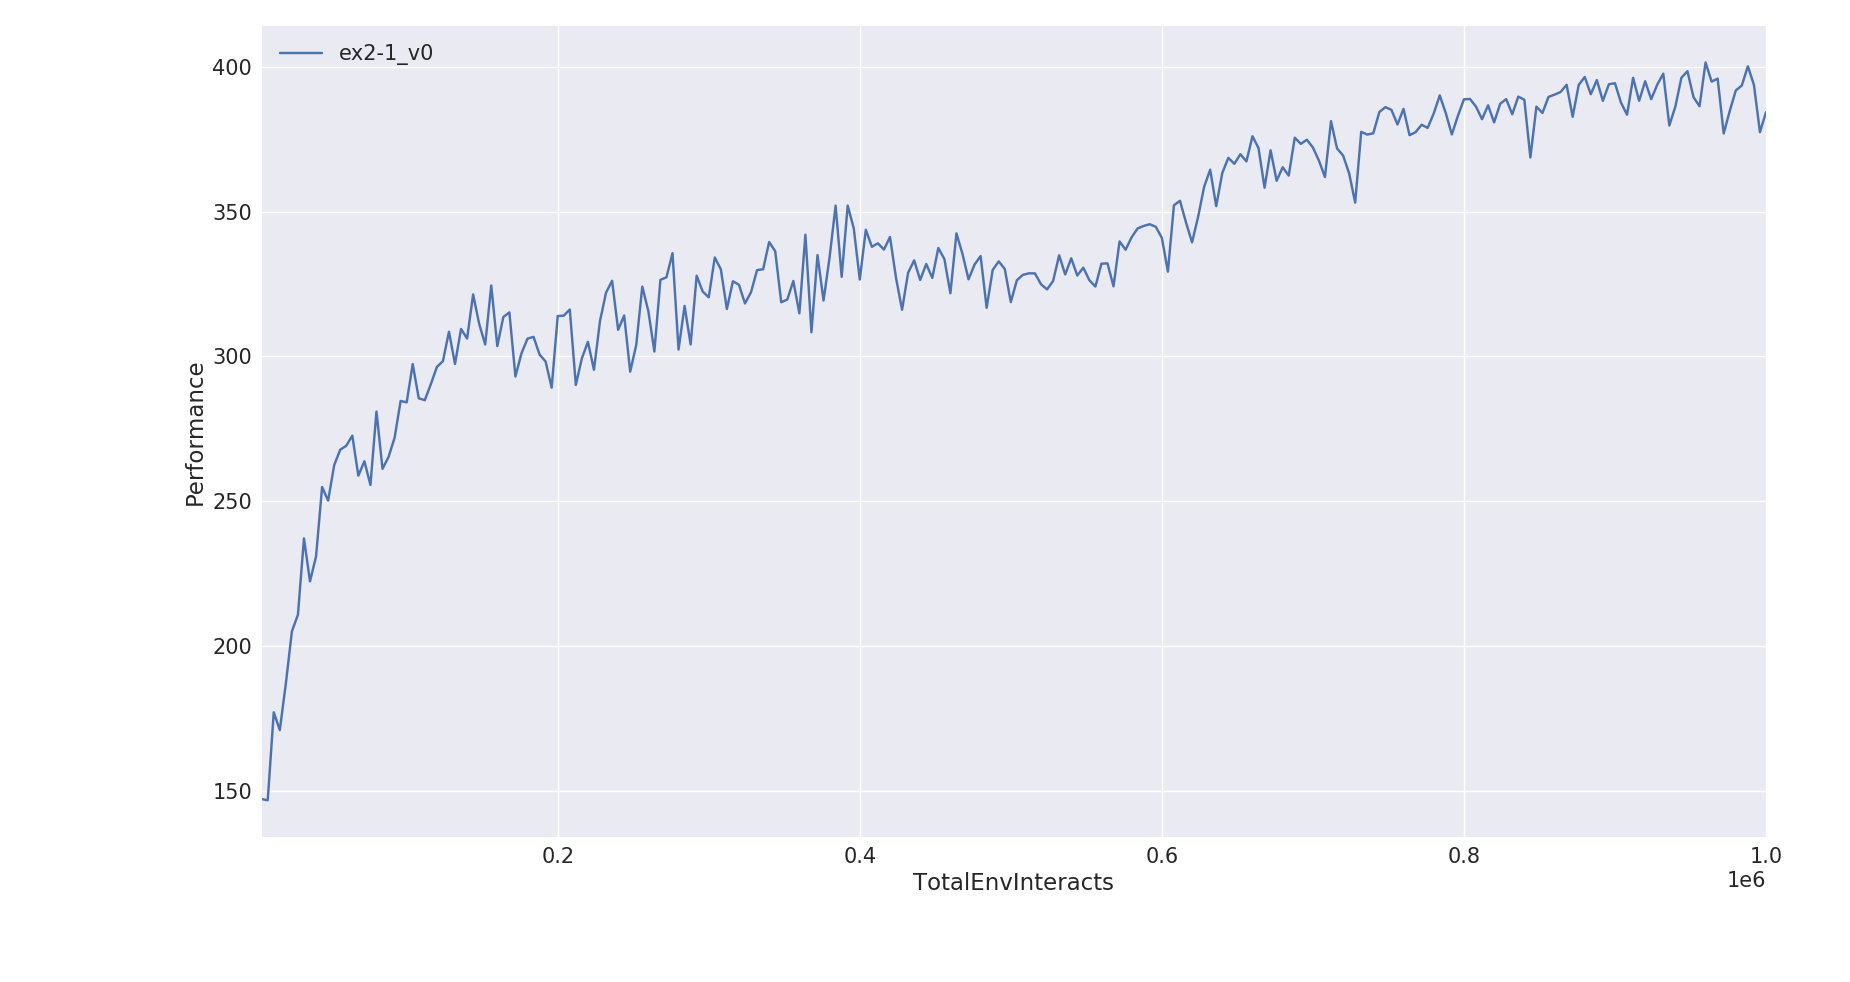
\includegraphics[width=0.32\textwidth]{../Img/spinningup_exercises/2_1/2_1_curve_v0_s20.png}
    \end{figure}

    The curve of v80 with different seeds are as follows:
    \begin{figure}[H]
        \centering
        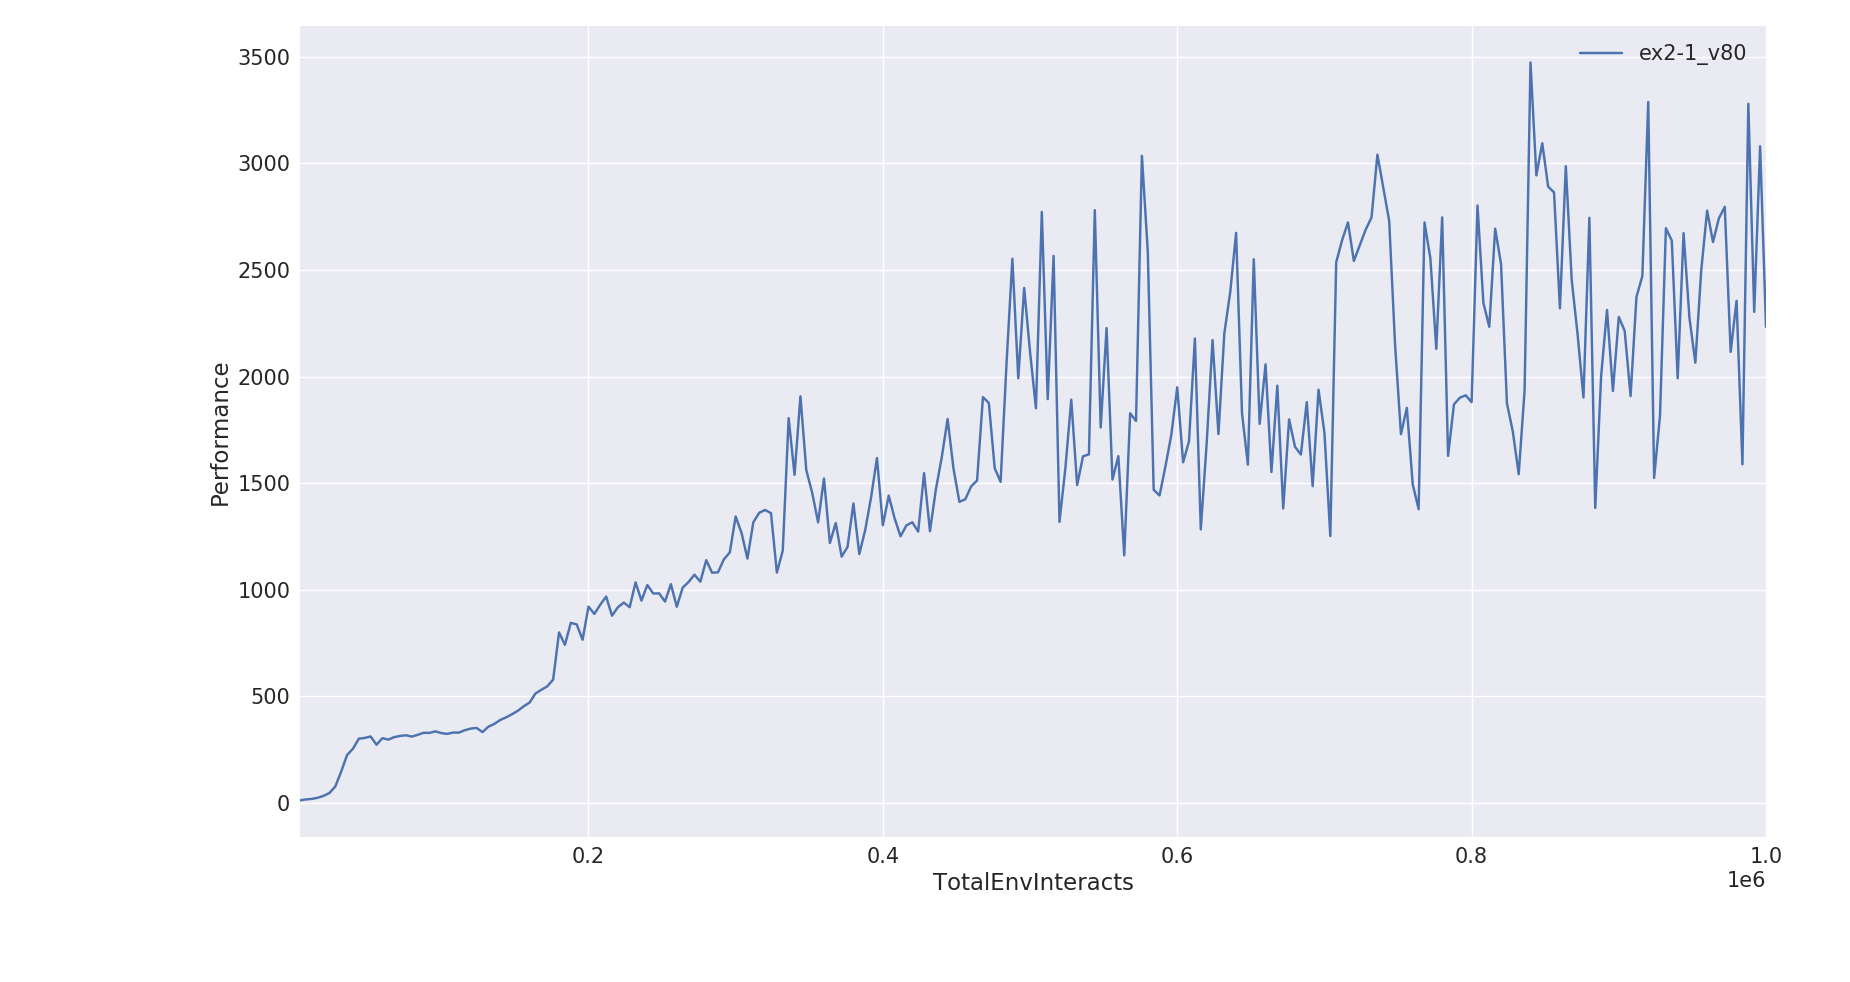
\includegraphics[width=0.32\textwidth]{../Img/spinningup_exercises/2_1/2_1_curve_v80_s0.png}
        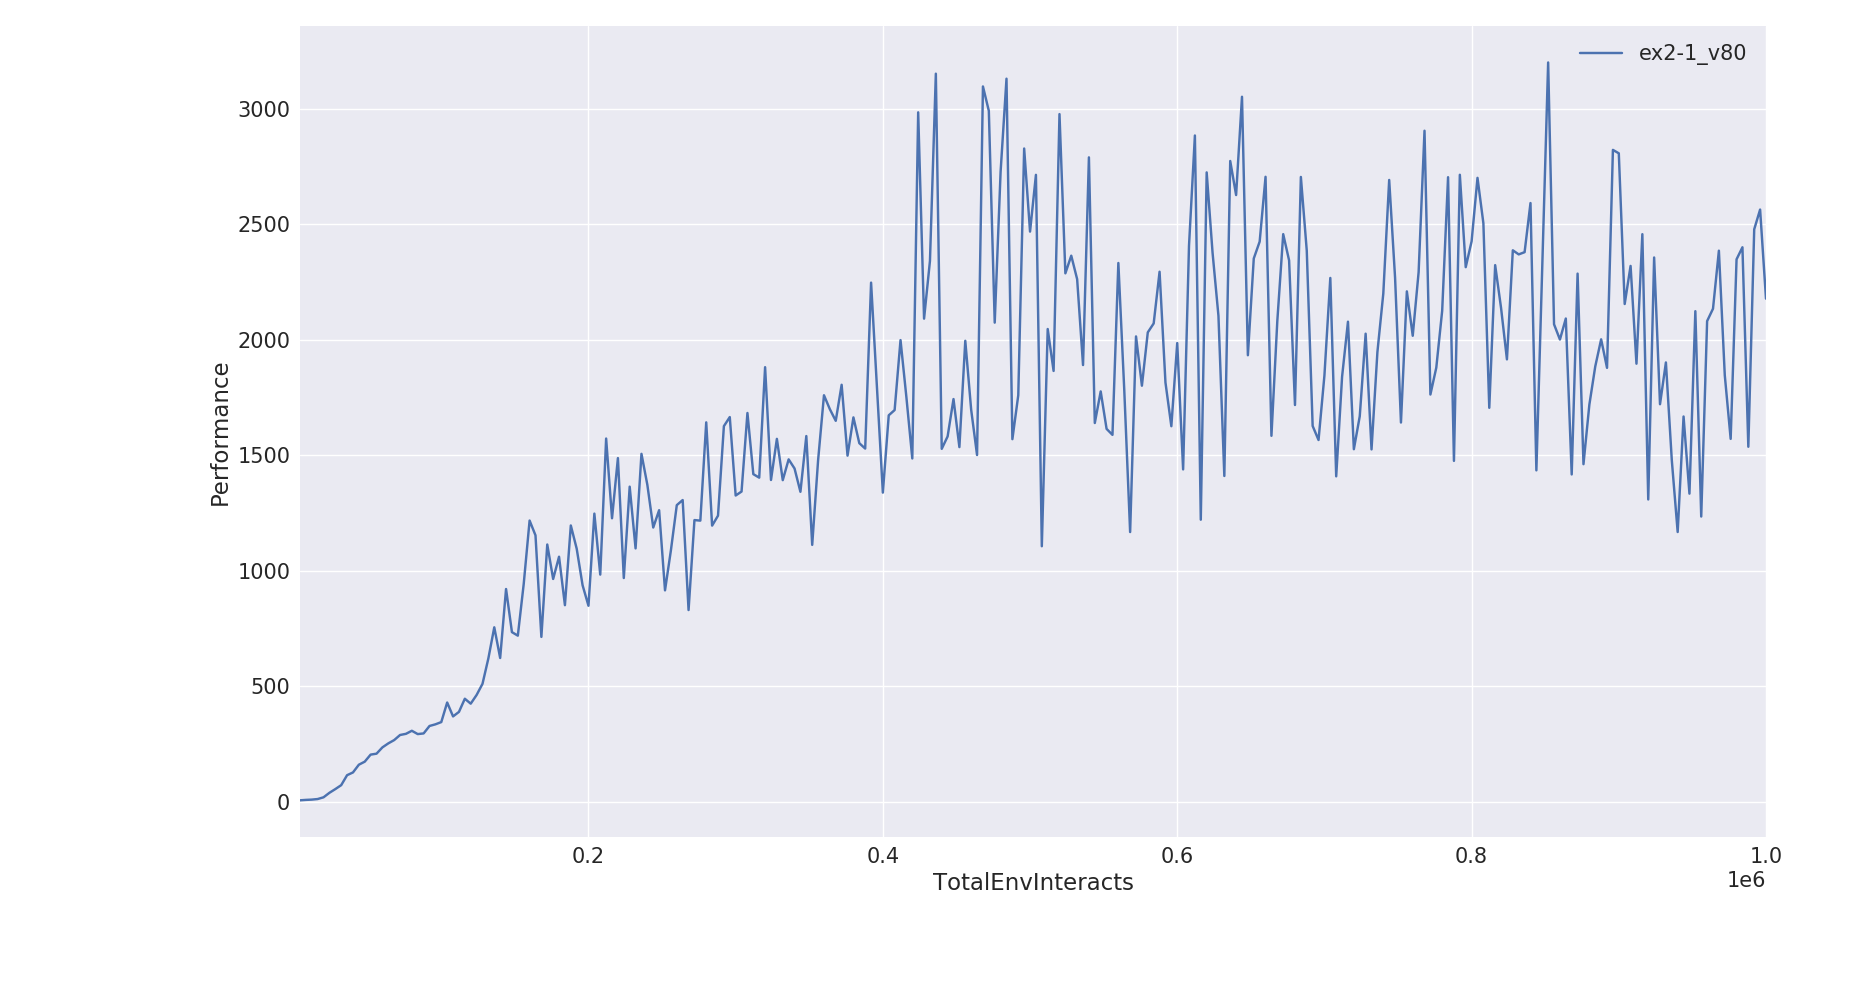
\includegraphics[width=0.32\textwidth]{../Img/spinningup_exercises/2_1/2_1_curve_v80_s10.png}
        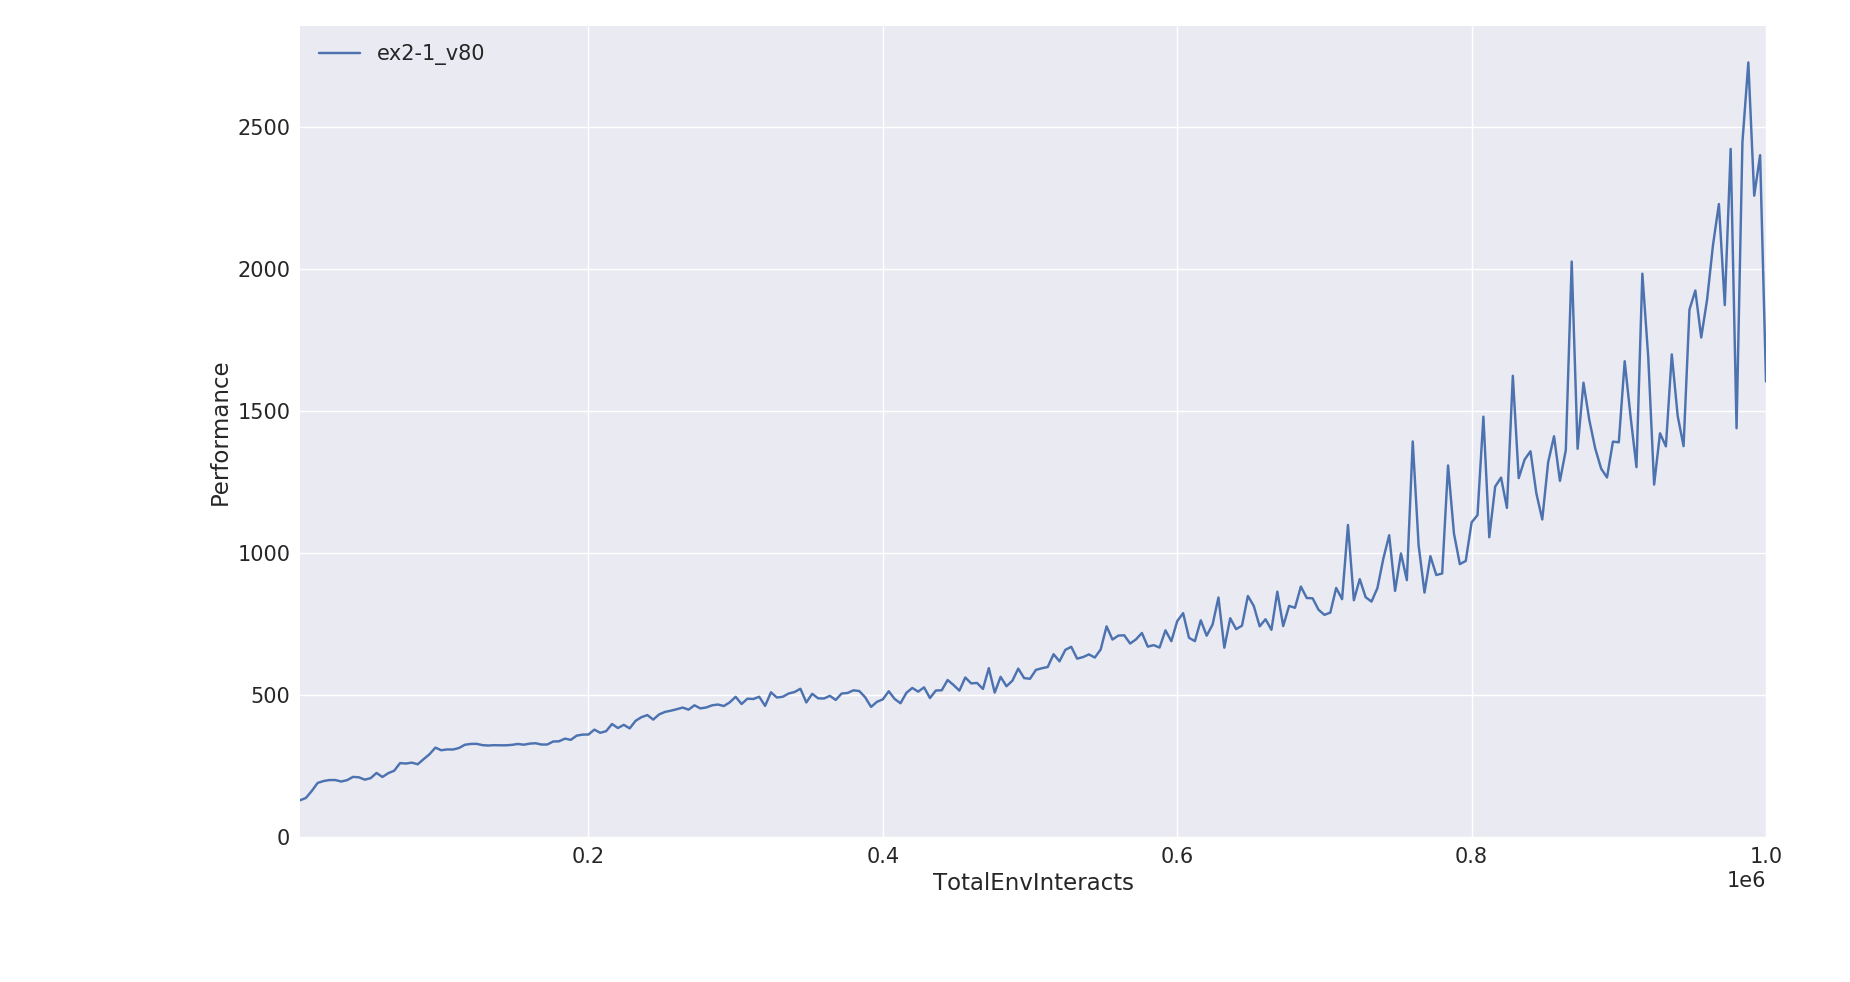
\includegraphics[width=0.32\textwidth]{../Img/spinningup_exercises/2_1/2_1_curve_v80_s20.png}
    \end{figure}

    The comparison between curve of v0 and v80, and their average and variance are as follows:
    \begin{figure}[H]
        \centering
        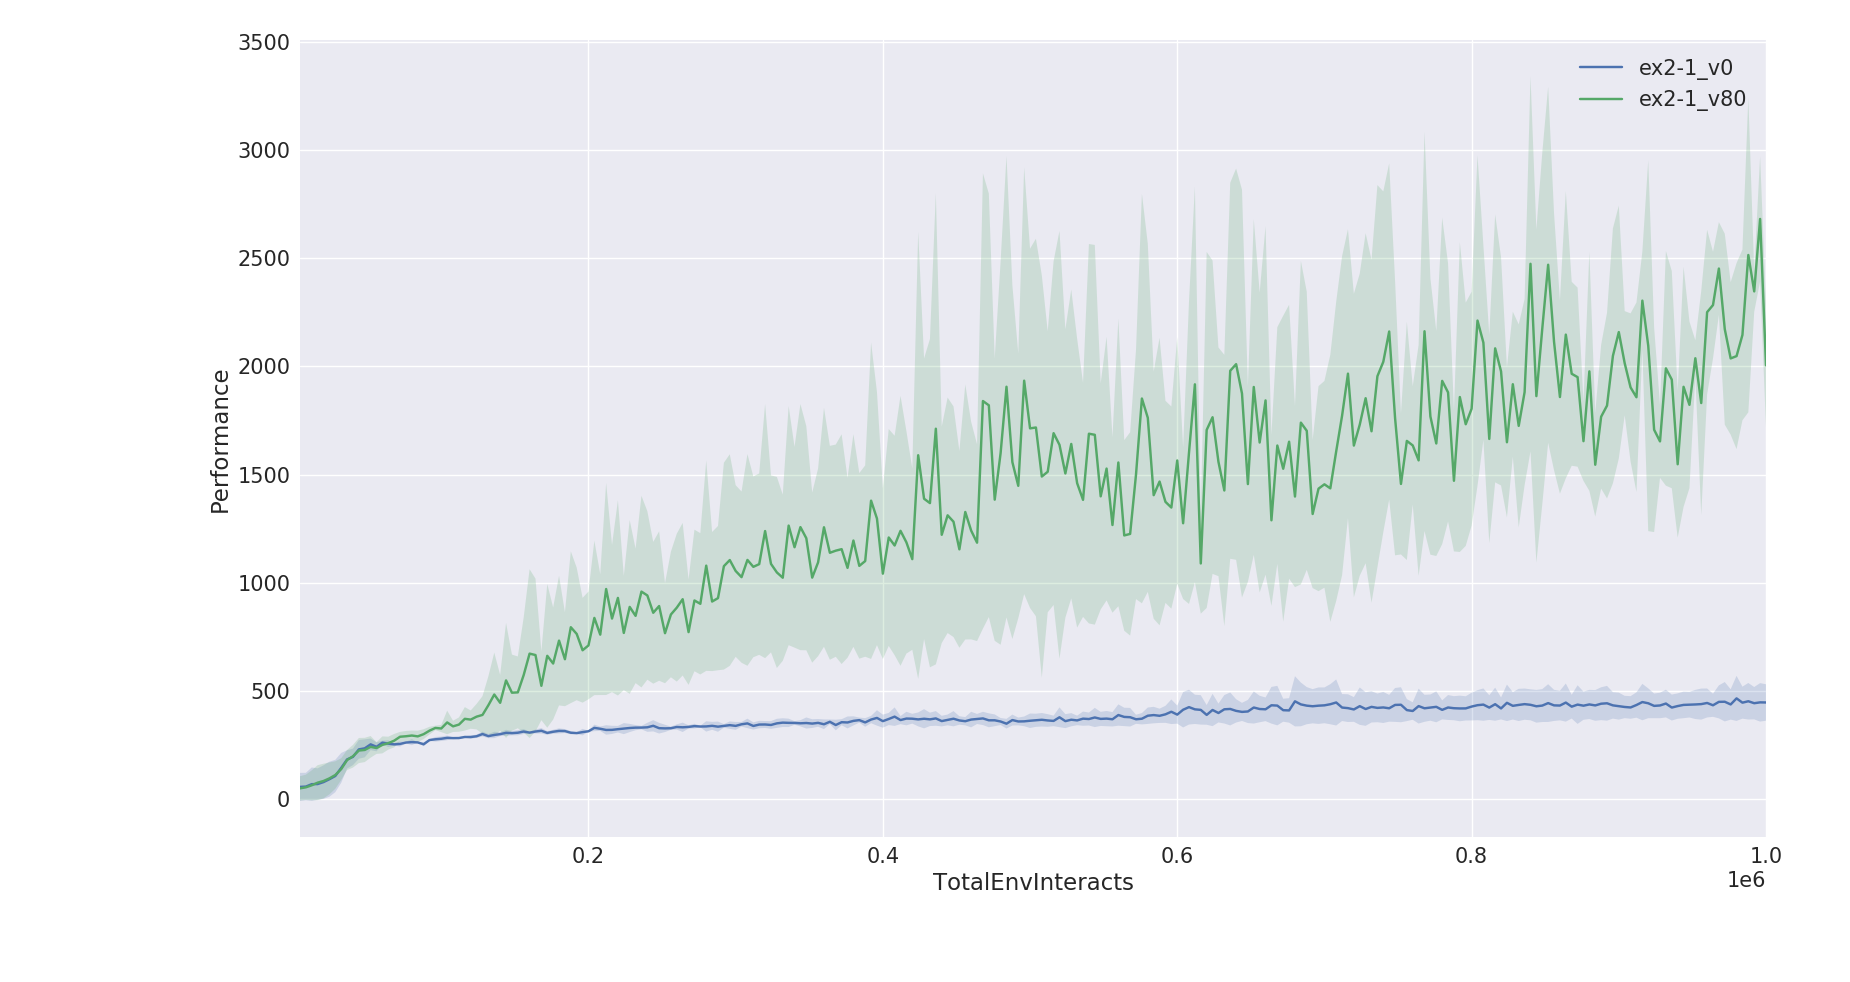
\includegraphics[width=\textwidth]{../Img/spinningup_exercises/2_1/2_1_curve_all.png}
    \end{figure}

    \item exercise 2\_2:
    The curve of the code without bug and with different seeds are as follows:
    \begin{figure}[H]
        \centering
        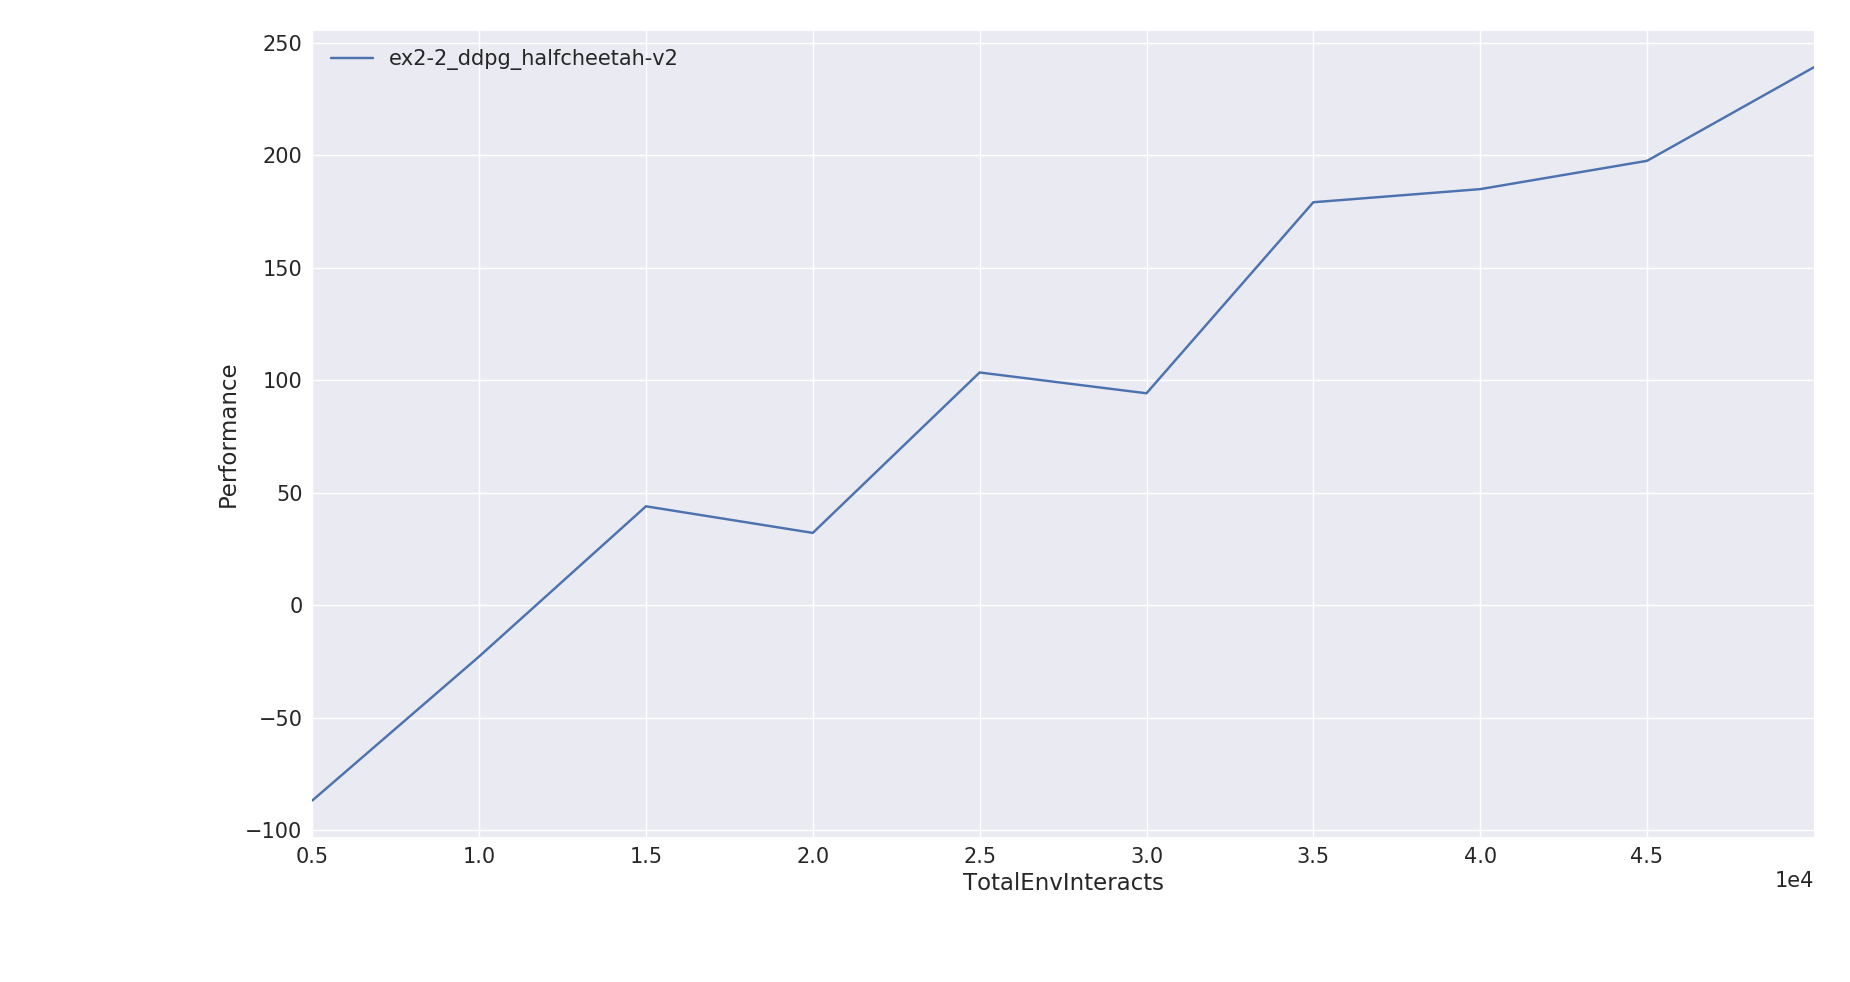
\includegraphics[width=0.32\textwidth]{../Img/spinningup_exercises/2_2/2_2_curve_s0.png}
        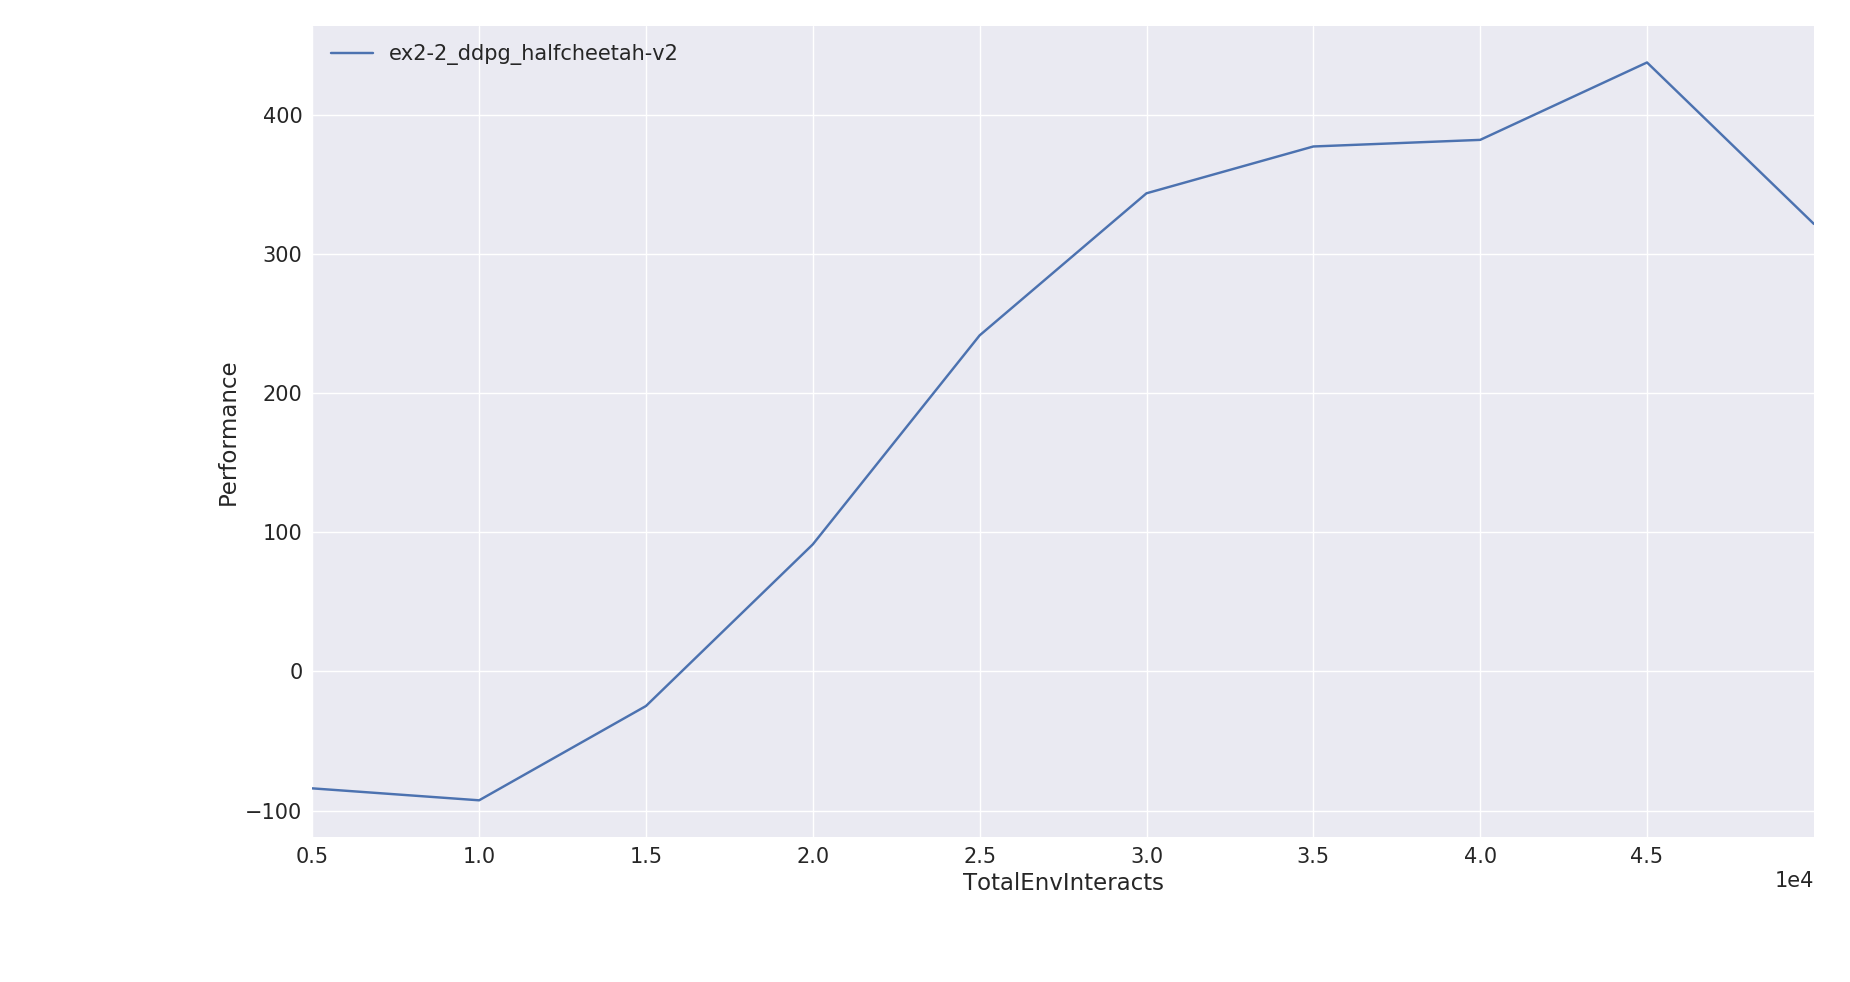
\includegraphics[width=0.32\textwidth]{../Img/spinningup_exercises/2_2/2_2_curve_s10.png}
        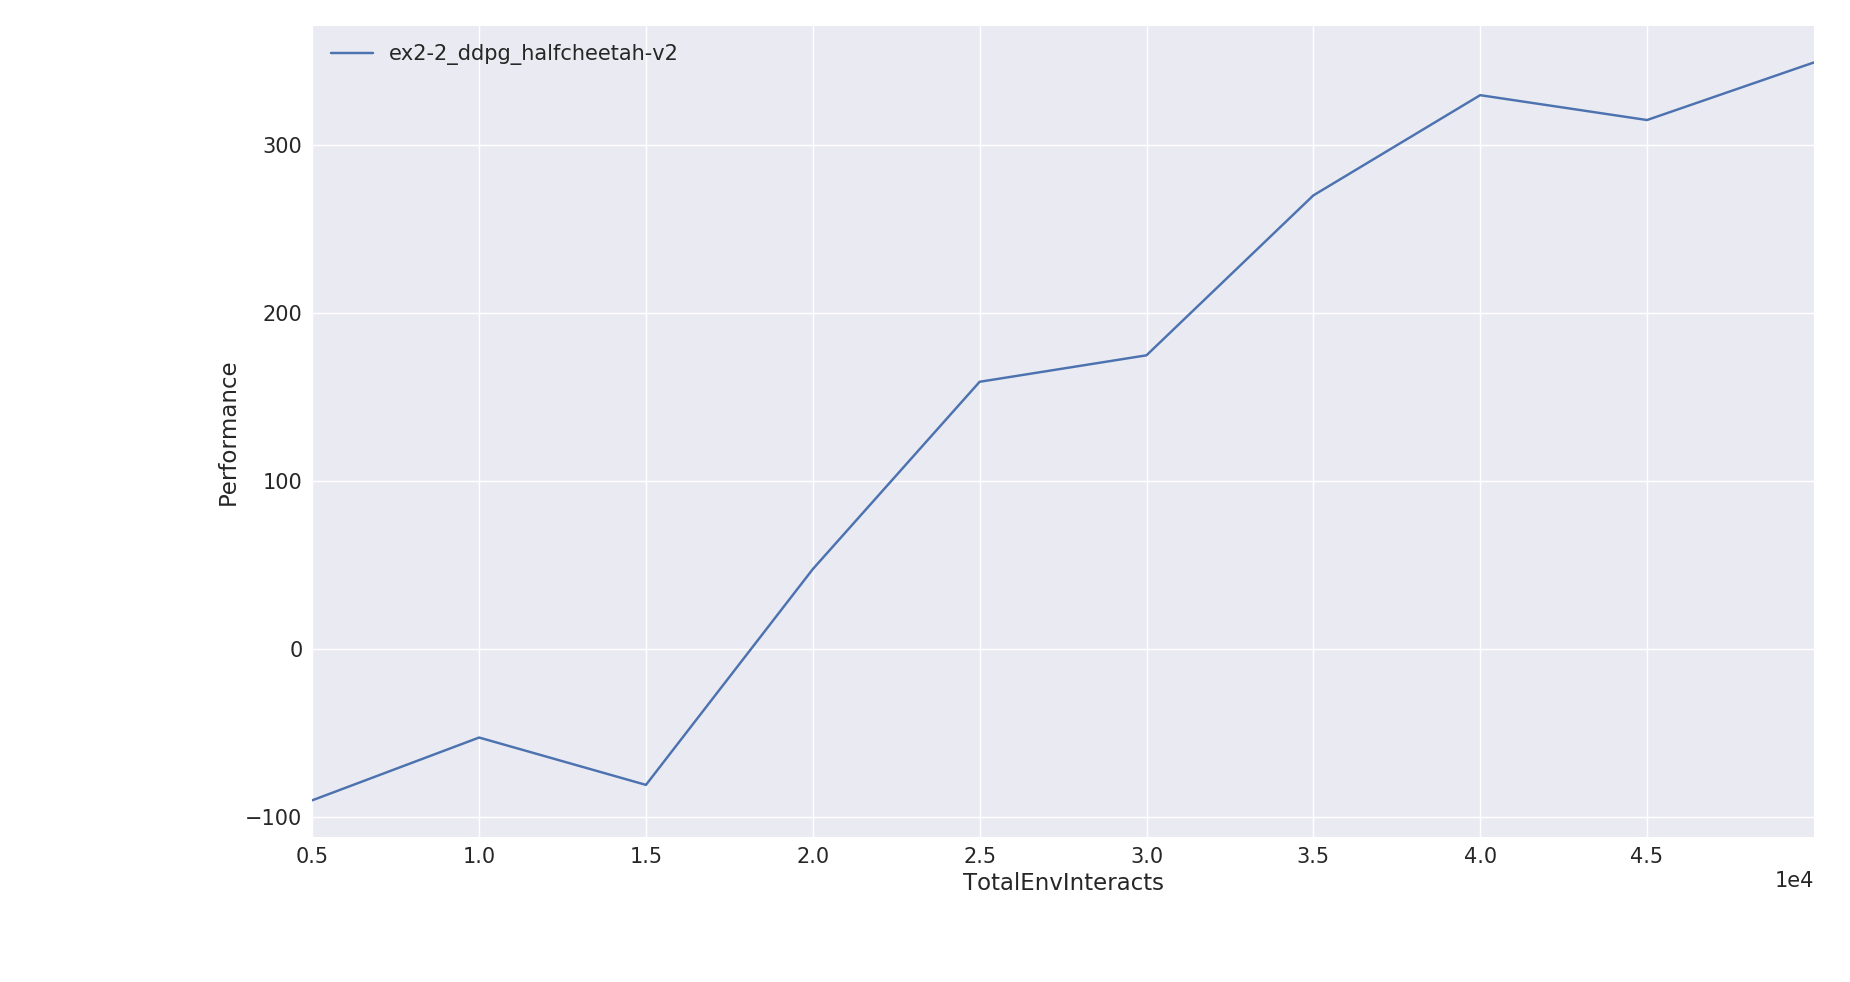
\includegraphics[width=0.32\textwidth]{../Img/spinningup_exercises/2_2/2_2_curve_s20.png}
    \end{figure}

    The curve of the code with bug and with different seeds are as follows:
    \begin{figure}[H]
        \centering
        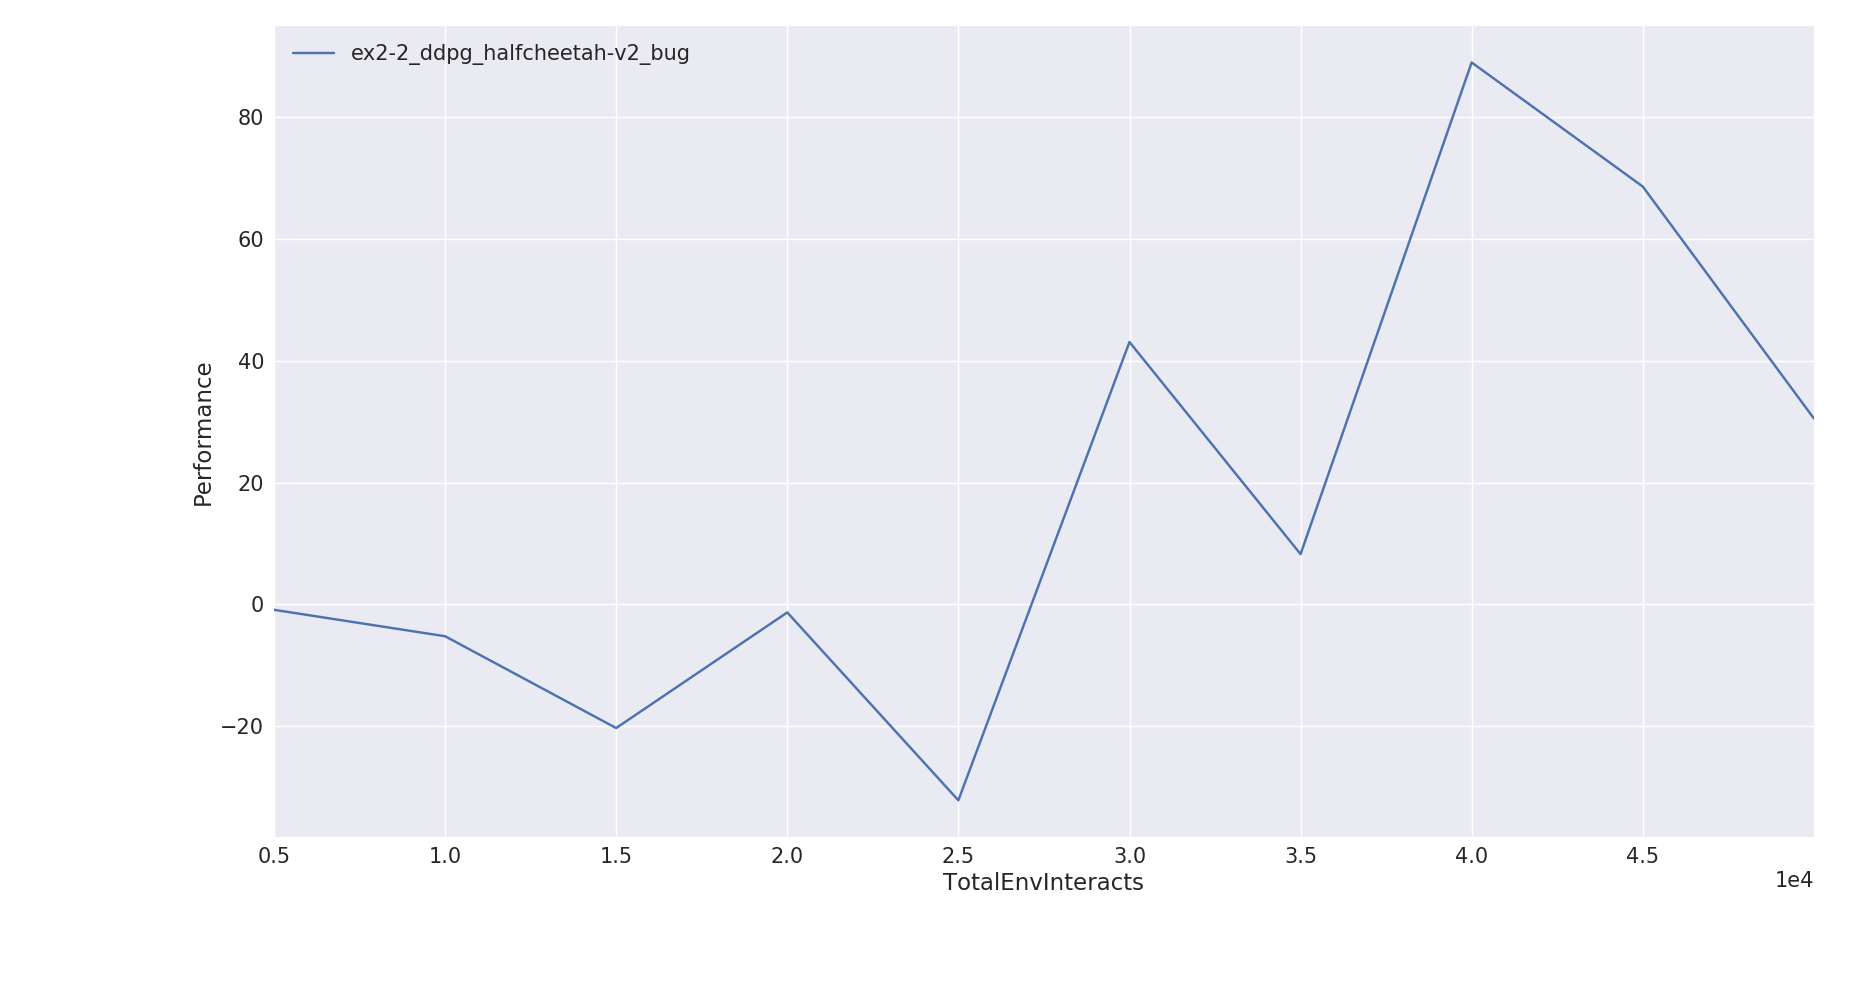
\includegraphics[width=0.32\textwidth]{../Img/spinningup_exercises/2_2/2_2_bug_curve_s0.png}
        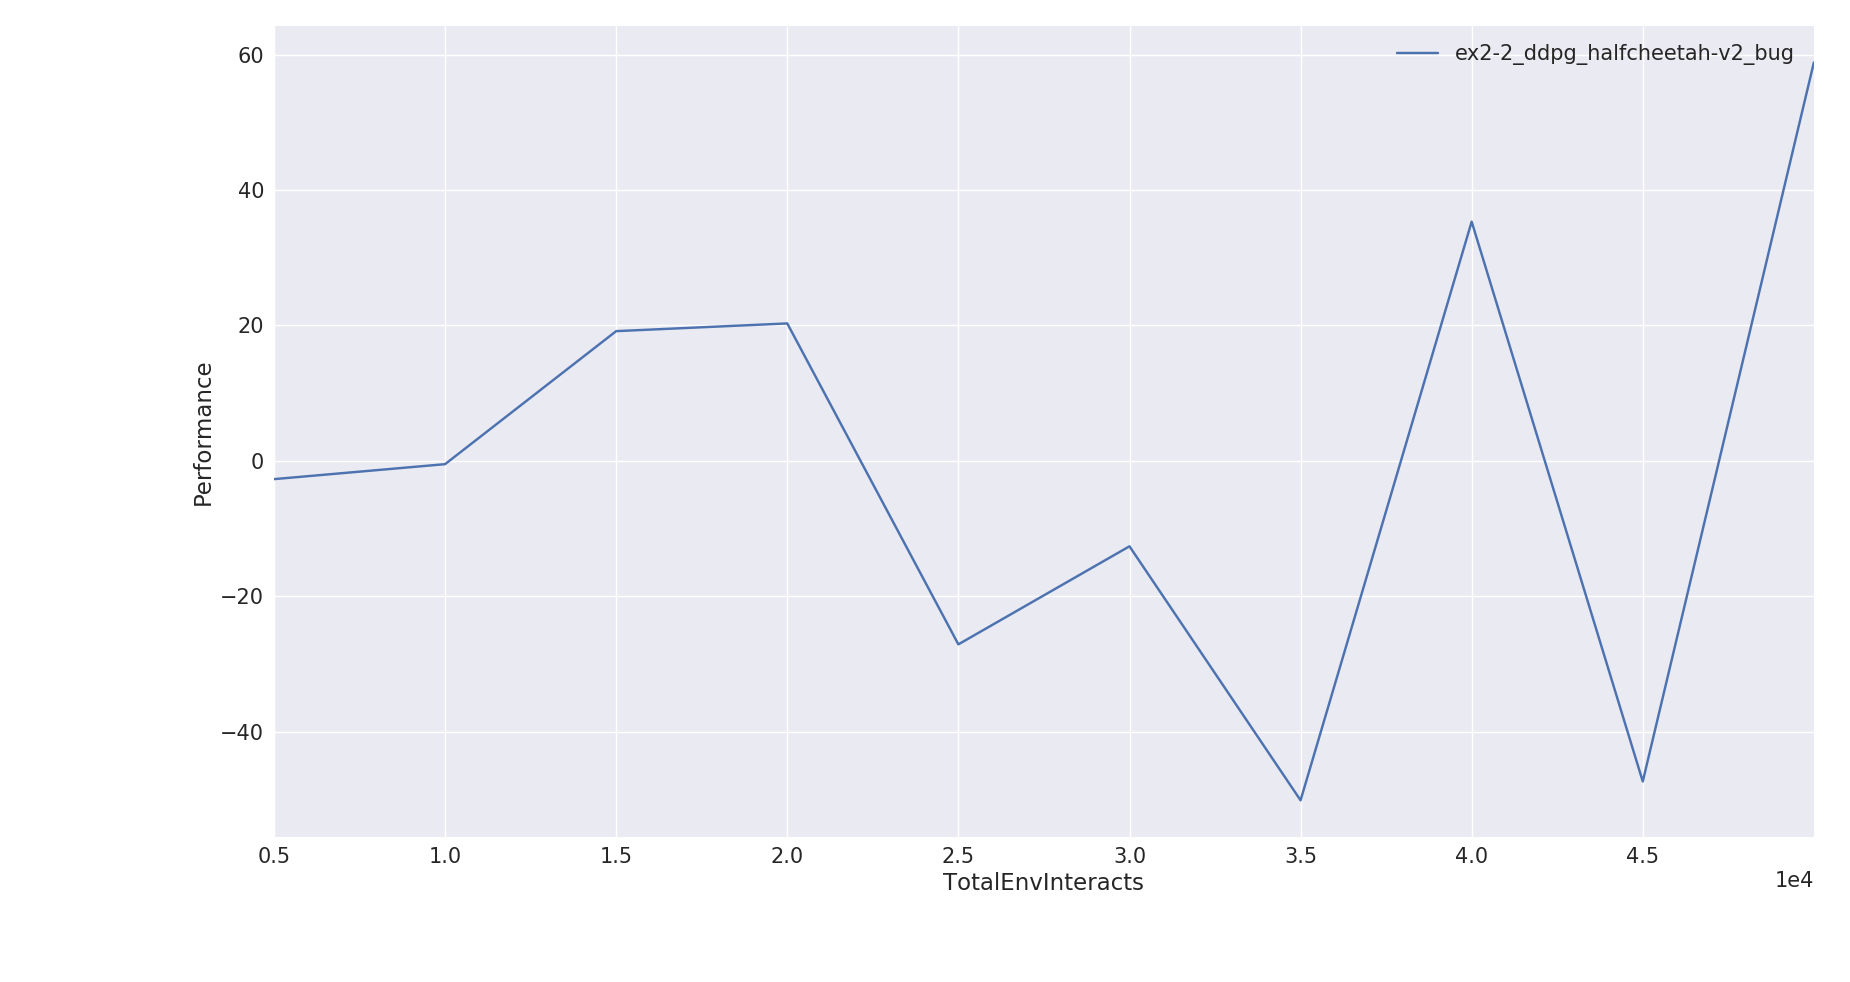
\includegraphics[width=0.32\textwidth]{../Img/spinningup_exercises/2_2/2_2_bug_curve_s10.png}
        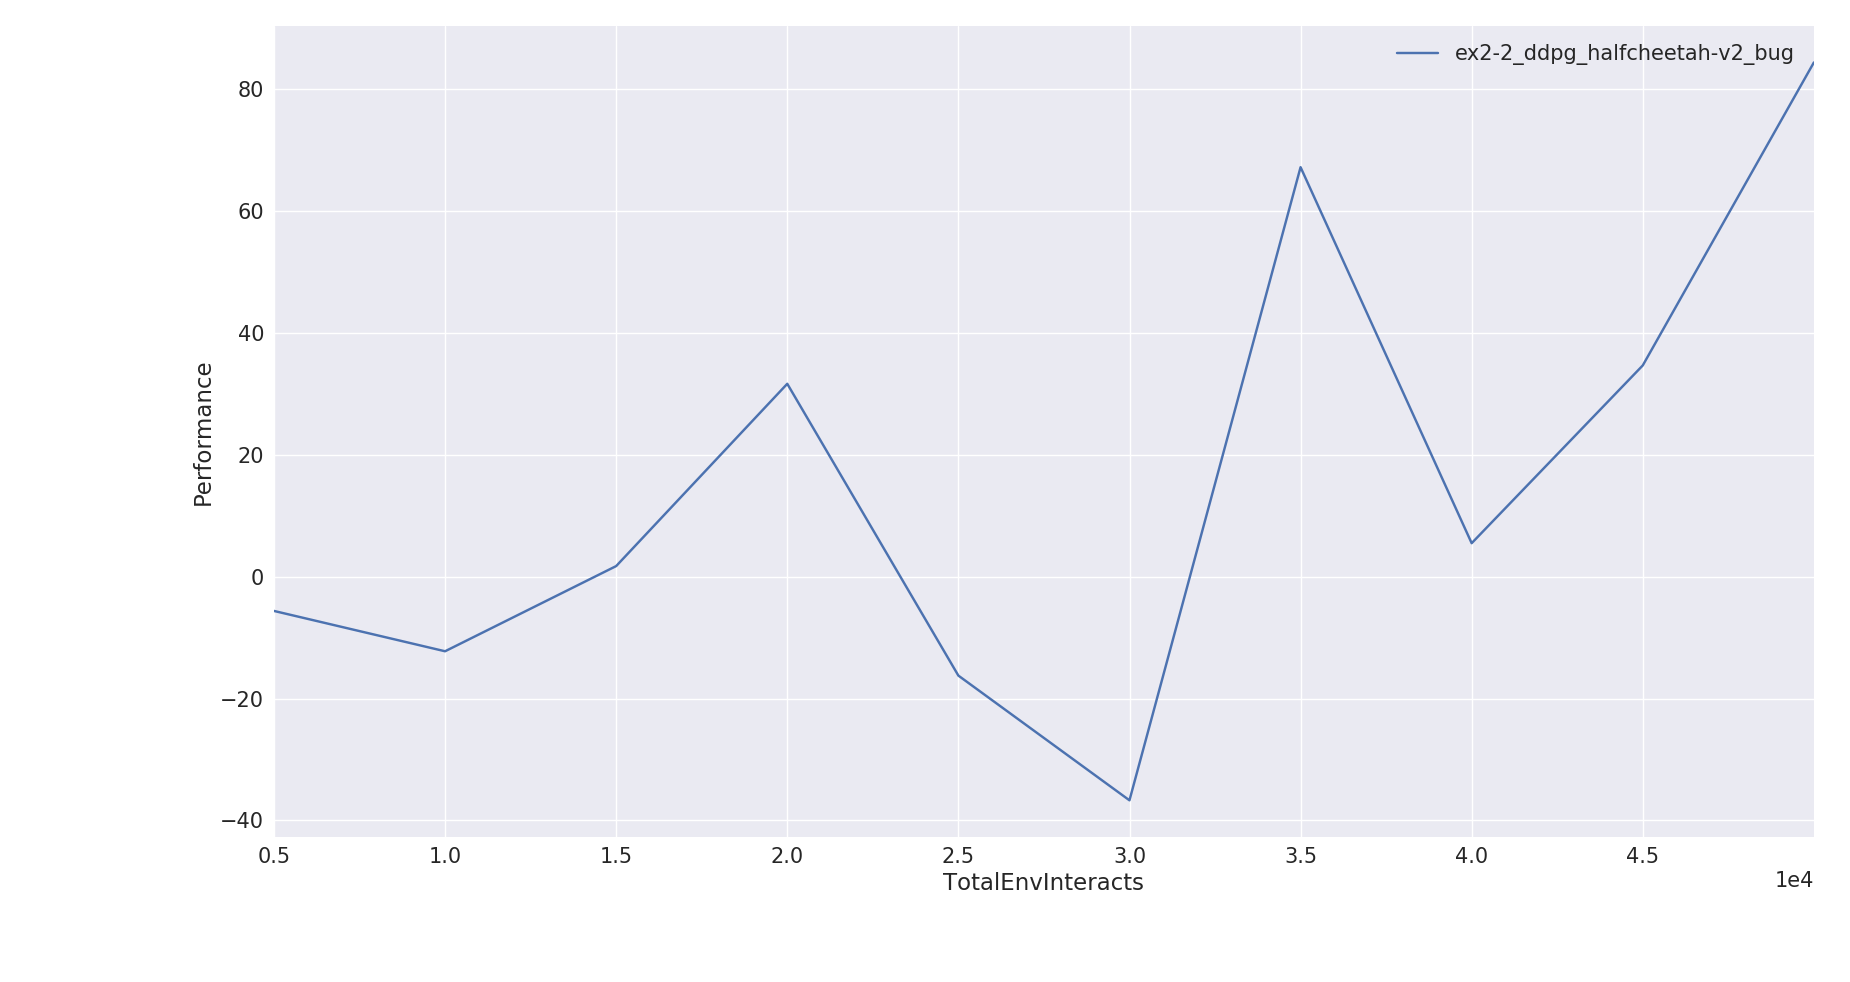
\includegraphics[width=0.32\textwidth]{../Img/spinningup_exercises/2_2/2_2_bug_curve_s20.png}
    \end{figure}

    The comparison between curve with and without bug, and their average and variance are as follows:
    \begin{figure}[H]
        \centering
        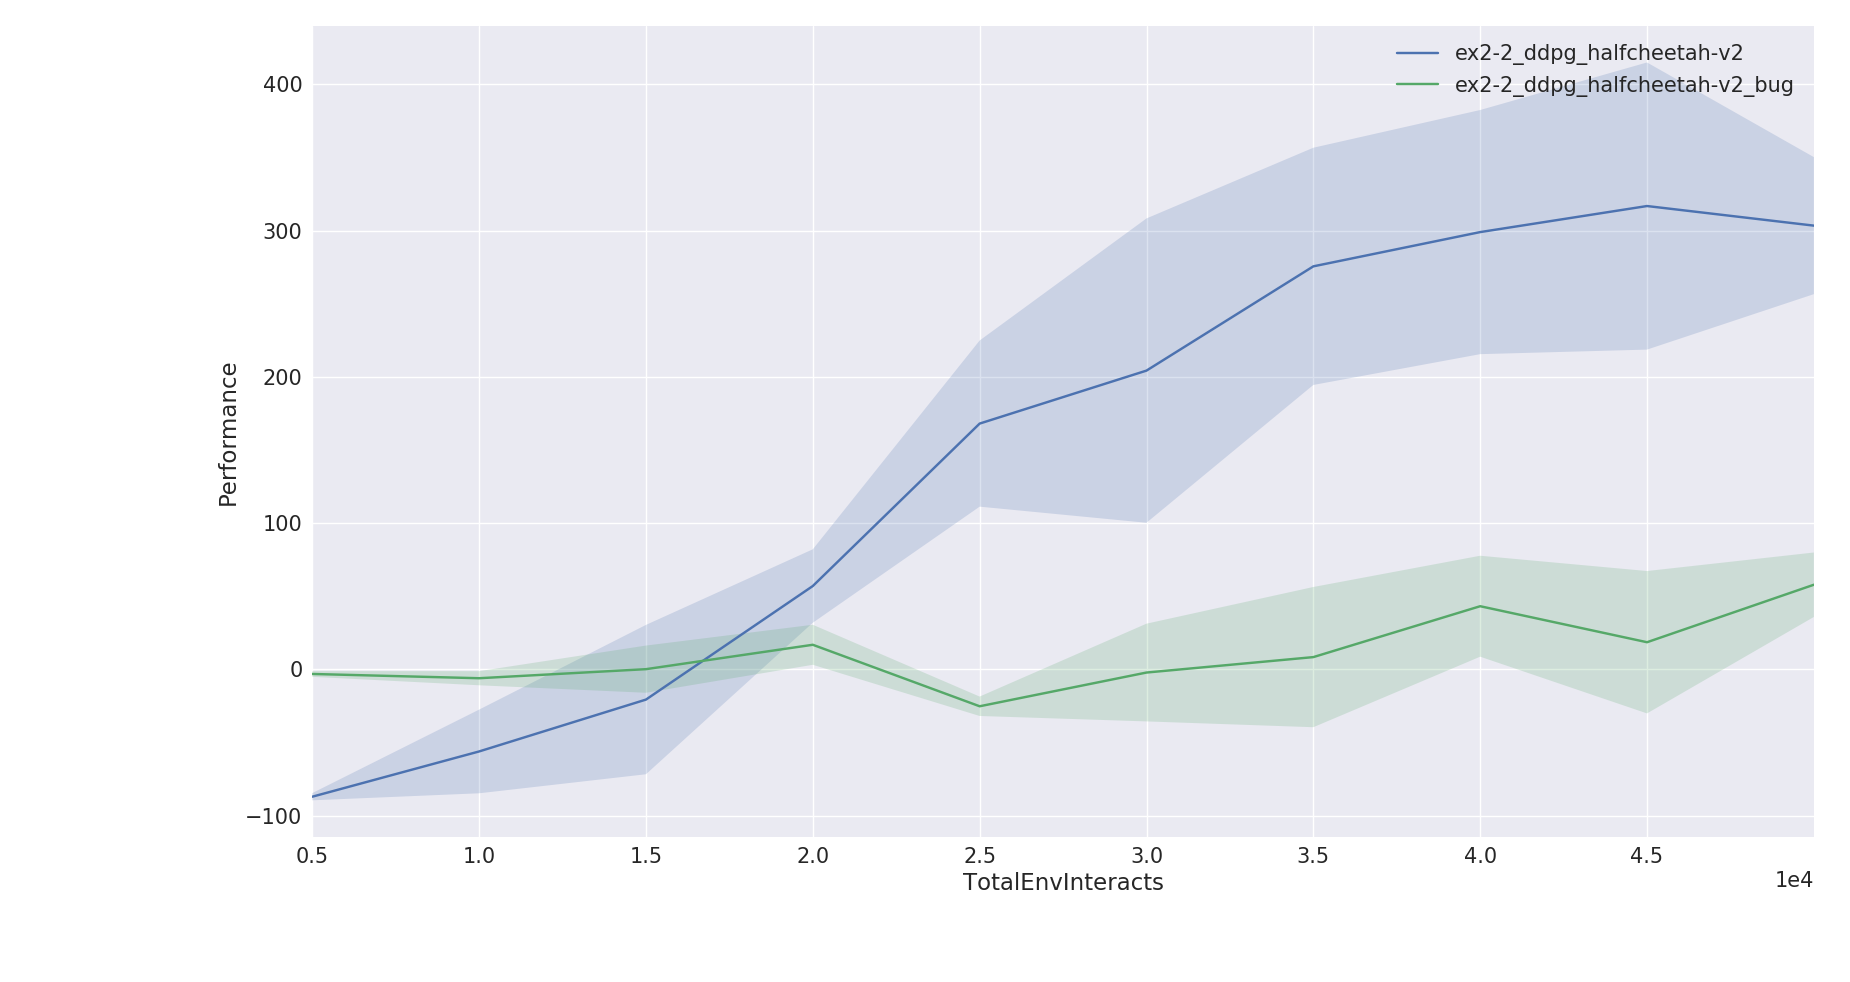
\includegraphics[width=\textwidth]{../Img/spinningup_exercises/2_2/2_2_curve_all.png}
    \end{figure}

    The code's bug is shown in the following figure:
    \begin{figure}[H]
        \centering
        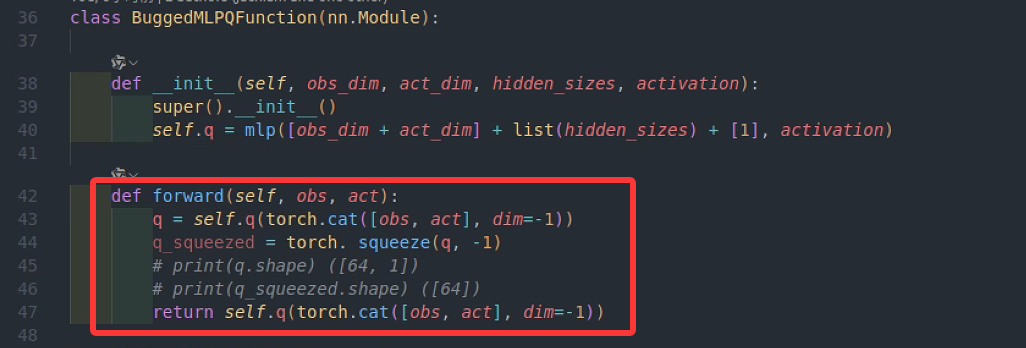
\includegraphics[width=\textwidth]{../Img/spinningup_exercises/2_2/2_2_mistake.png}
    \end{figure}


\end{itemize}



\end{homeworkProblem}

\newpage